\documentclass[./../../paper.tex]{subfiles}
\graphicspath{{\subfix{./../../figures/}}}

\begin{document}
% This section dives into the generative models that we explore in this thesis. They cover fundamentally different approaches to the counterfactual generation of process data. We apply the viability metric established in \autoref{sec:viability} to evaluate the performance of each model.


% Here, we attempt to capture the latent state-space of a model and use this space to sample counterfactual candidates.  Last, we explore a technique which does not require to optimise a differentiable objective function. Instead we use the viability measure as a fitness function and maximise the fitness of each counterfactual candidate.



All evolutionary algorithms use ideas that resemble the process of evolution. There are four broad categories: A \gls{GA} uses bit-string representations of genes, while \gls{GP} uses binary codes to represent programs or instruction sets. \gls{ES} require the use of vectors. Lastly, \gls{EP}, which closely resembles \gls{ES}, without imposing a specific data structure type\autocites{lambora_GeneticAlgorithmLiterature_2019,vikhar_Evolutionaryalgorithmscritical_2016}. Our approach falls into the category of \gls{GA}. We refer to the literature review of \citeauthor{vikhar_Evolutionaryalgorithmscritical_2016} for more insights into the field. The most vital concept in this category is the \emph{gene} representation. 

For the algorithm, we follow a rigid structure of the operations as outlined in \autoref{alg:evolutionary}. 
As \autoref{alg:evolutionary} shows, we define 5 fundamental operations. Initiation, Selection, Crossover, Mutation and Recombination. 
The core idea is to generate new individuals every generation while discarding those who are not deemed fit enough for the next iteration cycle. This optimization method differs from gradient-based methods such as \gls{DL}, because it does not require us to use differentiable functions. This makes evolutionary algorithms tremendously useful but also highly dependent on the composition of the fitness function.

% \needsalg{alg:pseudocode}{The basic structure of an evolutionary algorithm.}
\begin{algorithm}[htb!]
    \caption{The basic structure of an evolutionary algorithm.}
    \begin{algorithmic}
        \Require{Hyperparameters}
        \Ensure{The result is the final population}
        \State $population \gets \text{INIT } population$;
        \While{not $termination$}
        \State $parents \gets \text{SELECT } population$;
        \State $offspring \gets \text{CROSSOVER } parents$;
        \State $mutants \gets \text{MUTATE } offspring$;
        \State $survivors \gets \text{RECOMBINE } population \cup mutants$;
        \State $termination \gets \text{DETERMINE } termination$
        \State $population \gets survivors$
        \EndWhile
    \end{algorithmic}
    \label{alg:evolutionary}
\end{algorithm}

The initiation operator refers to the creation of the initial set of candidates for the selection process in the first iteration of the algorithm. Often, this amounts to the random generation of individuals.  However, choosing among a subset of the search space can allow for a faster convergence. 

\begin{figure}[htbp]
    \centering

    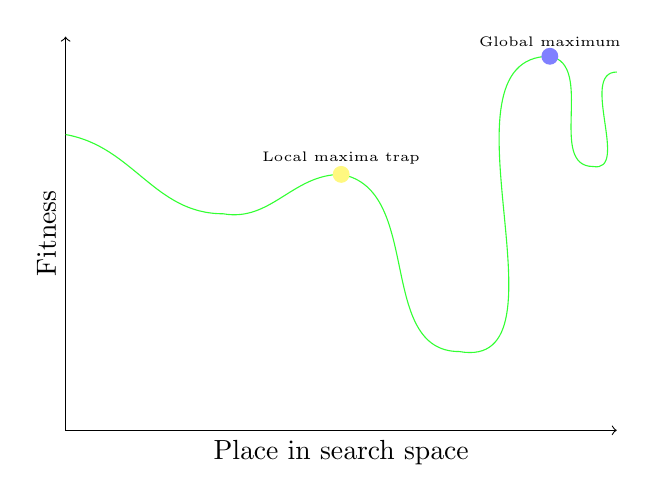
\begin{tikzpicture}
        %Opsætning af koordinater
        \coordinate (bottom) at (5,1);
        \coordinate (lmen) at (2 , 2.75);
        \coordinate (lman) at (3.5 , 3.25);
        \coordinate (rmen) at (6.7,3.35);
        \coordinate (rman) at (6.15,4.75);
        \coordinate (lkant) at (0,3.756);
        \coordinate (rkant) at (7,4.55);
        \coordinate (o) at (0,0);
        \coordinate (x) at (7,0);
        \coordinate (y) at (0,5);
        
        %tegn grafsystem
        \draw [<->] (y) -- node [rotate=90, above] {Fitness} (o) -> node [below] {Place in search space} (x);
        
        % Selve energikurven
        % \draw [green!80] plot [smooth, tension=.2] coordinates {(lkant) (lmen) (lman) (bottom) (rman) (rmen) (rkant)};
        \draw [green!80, in=180, out=0, tension=.1]
          (lkant)[out=-10] to (lmen) to (lman) to (bottom) to (rman) to (rmen) to (rkant);
        
        %lagels og sådant
        
        % \filldraw[color = red!50] (bottom) circle  (0.1) node [below,color=black] {\tiny Local minima};
        % \filldraw [color = red!50] (lmen) circle (0.1) node [below,color=black] {\tiny Local minima};
        % \filldraw [color = red!50] (rmen) circle (0.1) node [below,color=black] {\tiny Local minima};
        \filldraw [color = yellow!50] (lman) circle (0.1) node [above,color=black] {\tiny Local maxima trap};
        \filldraw [color = blue!50] (rman) circle (0.1) node [above,color=black] {\tiny Global maximum};
        \end{tikzpicture}
        \caption{Schematic example showing various local optima.}

        \label{fig:localmax}

\end{figure}

The selection operator chooses a set of individuals among the population according to a selection procedure. These individuals go on to act as material to generate new individuals. This operator can strongly influence the level with which the algorithm explores the search space. For instance, if an algorithm only selects the best individuals it is easy to get stuck within an local maximum. \autoref{fig:localmax} displays why local maxima should be avoided. Mainly, if we get stuck, we may not be able to find the absolute best solution.

Within the crossover procedure, we select random pairing of individuals to pass on their characteristics. We can often generate at least two additional offsprings, if we have two parents and just reverse the operation.

Mutations introduce random pertubations to the offsprings. This extends the search space beyond what is available by the parents.  

The Recombination operation decides which individuals remain in the population for the next iteration\footnotemark[1]. This operator-type is a second source that determines the exploration space of the evolutionary algorithm. For instance, if we only allow the best 10 individuals to move on to the next iteration and only select the top 3 individuals for the crossover phase, we quickly converge towards one solution. Hence, both operators interact, which is why the literature often treat these operations as identical. However, splitting them allows us to control the number of sampled off spring and the population size separately.  








We name the strict selection of the best individuals among the offsprings and the previous population \emph{Fittest-Survivor-Recombination}. This recombiner strictly optimizes the population and is susceptible to getting stuck in local minima. 
In contrast, we name the addition of the top-k best offsprings to the initial population \emph{Best-of-Breed-Recombination}. The former will guarantee, that the population size remains the same across all iterations but is prone to local optima. Furthermore, we propose one additional recombination operator. The operator selects the new population in a different way than the former recombination operators. Instead of using the viability directly, we sort each individual by every viability component, separately. This approach allows us to select individuals regardless of the scales of every individual viability measure. We refer to this method as \emph{Ranked-Recombination}. 

% The second approach is similar. However, this time we sort each individual by their pairwise-pareto dominance. In other words, we decide selecting individuals by selecting the individuals first, who have the highest delta without reducing the feasibility. Then, those with the highest feasibility, without reducing sparsity and so on. All individuals that fall through the cut-off point are discarded\attention{Change num survivors to cut-off point.}.   
% We refer to this approach as \emph{Ranked-Pareto-Recombination}. 

% The difference between \emph{Ranked-Pareto-Recombination} and \emph{Ranked-Recombination} is subtle. We show this in \autoref{fig:ranked-pareto}.

% \needsfigure{fig:ranked-pareto}{The difference between both approaches on two arbitrary dimensions. It shows the number that are selected on the pareto frontier and those selected by sorting. The selected individuals are marked by a cross.}
% TODO: Create a picture based on some examples


\footnotetext[1]{We have to point out that in the literature, recombination is often synonymous with crossover. Both steps are similar in their filtering purpose. However, the selector filters potential parents while the recombiner filters the population. However, in this thesis recombination refers to the update process which generates the next population.}

\end{document}